\textbf{Cited from} \href{https://steemit.com/monero/@luigi1111/understanding-monero-cryptography-privacy-introduction}{XMR crypto blog series} by \href{https://github.com/luigi1111}{luigi1111}.\par

\begin{displayquote}
This is part two of a series of unknown size; it'll be done when it's done. Part one is \href{https://steemit.com/monero/@luigi1111/understanding-monero-cryptography-privacy-introduction}{here}.\\\\
Part one focuses on the basics: ECC, the particular curve, private and public "keys", and a bonus section on how Monero addresses are generated. \\\\
Note: Monero is based on the \href{https://cryptonote.org/whitepaper.pdf}{Cryptonote protocol} -- though it has diverged and will continue to diverge -- along with numerous other coins; much of this series applies equally well to the others with some caveats. Monero is easily the largest and most active Cryptonote-based project.
\end{displayquote}

Hello! I'm an autodidact enthusiast of cryptography, particularly in relation to the crypto-currency \href{https://getmonero.org/}{Monero}. Naturally, you should not assume everything I say is correct, and I hope any egregious errors are pointed out so I can fix them (and help my own understanding). Just calling me an idiot is fine too.

\begin{figure}[H]
	\centering
	
\includegraphics[width=0.4\linewidth]{./images/blog-series/xmr-crypto-luigi1111/idiot-doctor.jpg}
\end{figure}

Monero's tagline is ``Secure, Private, Untraceable.'' Secure could refer to a number of facets of a crypto-currency, but here we are only particularly interested in security relating to privacy/anonymity. These articles will be looking at how Monero achieves ``privacy'', that is unlinkability and untraceability, with references to security where appropriate. This article focuses on some concepts, which will hopefully make understanding the others easier. Without further ado, let's get into it!

\subsection{What is Elliptic Curve Cryptography?}
Alright, so what is ECC? From \href{https://en.wikipedia.org/wiki/Elliptic_curve_cryptography}{Wikipedia}: ``\textbf{Elliptic curve cryptography (ECC)} is an approach to \href{https://en.wikipedia.org/wiki/Public-key_cryptography}{public-key cryptography} based on the \href{https://en.wikipedia.org/wiki/Algebraic_structure}{algebraic structure} of \href{https://en.wikipedia.org/wiki/Elliptic_curve}{elliptic curves} over \href{https://en.wikipedia.org/wiki/Finite_field}{finite fields}.''

Now, what does that mean? \emph{I have no idea.}

More seriously, let's go through it:
	\begin{enumerate}
		\item Public-Key Cryptography, or asymmetric cryptography, uses a pair of keys instead of a single private key as in symmetric cryptography (e.g., \href{https://en.wikipedia.org/wiki/Advanced_Encryption_Standard}{AES}): a public key, to be given out to "the world"; and a private key, to be always kept secret. To be secure, it must be hard intractable to figure out the private key given the public key; to be usable it must be easy to calculate the public key given the private key. ECC relies on the \href{https://en.wikipedia.org/wiki/Discrete_logarithm}{ECDLP} for its security. \textbf{Takeaways: public/private key pair; private->public is easy, but public->private is "impossible".}
		\item ``algebraic structure of elliptic curves'': \emph{What is this???} It is a plane curve satisfying \(y^2=x^3+ax+b\). It might look something like \figurename~\ref{fig-xmr-crypto-luigi1111-elliptic-curve-eg}\\
			\emph{Who cares?} Right, probably no one. In case someone does, there's a wealth of articles (many related to Bitcoin) out there that explain in detail how they work, how addition is possible, etc. Some examples: \href{http://andrea.corbellini.name/2015/05/17/elliptic-curve-cryptography-a-gentle-introduction/}{A, B, C (a series itself)}. Numerous videos are out there too, if you're into that. \textbf{Takeaways: none, this funny-looking curve will not help you understand and isn't even how Monero's curve looks.}
		\item ``over finite fields'': this just means curve points are taken modulo some (large, prime) number. Everyone is familiar with modular addition and subtraction at least (even if they've never heard the word) due to our time-keeping. \emph{If it is 10am, what time will it be in 5 hours?} \textbf{Congrats, you just did modular addition.} An elliptic curve over a finite field might look something like \figurename~\ref{fig-xmr-crypto-luigi1111-elliptic-curve-GF-eg}\\
			\textit{Whoa, that looks odd.} Yes, it does. \textbf{Takeaways: none. Actually, note how the points are ``reflected'' over an invisible line in the center.}
	\end{enumerate}
\begin{figure}[H]
	\begin{subfigure}{0.4\linewidth}
		\centering
		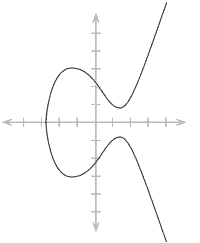
\includegraphics[width=0.6\linewidth]{./images/blog-series/xmr-crypto-luigi1111/elliptic-curve-eg.png}
		\caption{An example of elliptic curves}\label{fig-xmr-crypto-luigi1111-elliptic-curve-eg}
	\end{subfigure}
	\begin{subfigure}{0.55\linewidth}
		\centering
		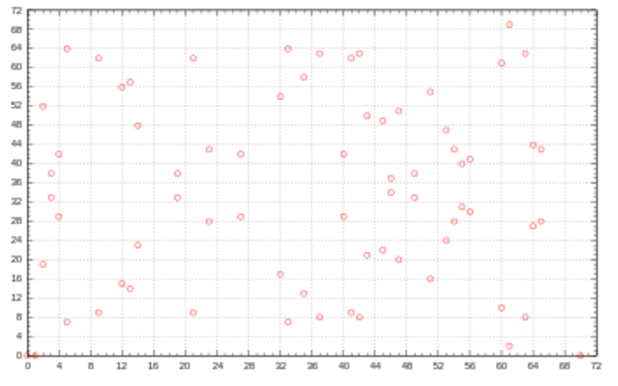
\includegraphics[width=0.8\linewidth]{./images/blog-series/xmr-crypto-luigi1111/elliptic-curve-GF-eg.png}
		\caption{An example of elliptic curves}\label{fig-xmr-crypto-luigi1111-elliptic-curve-GF-eg}
	\end{subfigure}
\end{figure}
A primary benefit of using ECC vs something like \href{https://en.wikipedia.org/wiki/RSA_(cryptosystem)}{RSA} is that keys are much smaller for similar security levels.

\subsubsection{I believe the only things you need to know to proceed are:}
	\begin{enumerate}
		\item A point on the curve can be added to or subtracted from another point, or itself.
		\item A point cannot be multiplied or divided by another point.
		\item Adding a point to itself allows ``scalar multiplication'', \textbf{which is where the magic happens}.
	\end{enumerate}

Subtracting a point from itself isn't very useful, as it'll just return the ECC equivalent of 0. Division by integer isn't possible (the equivalent modular operation -- modular multiplicative inverse -- is, but only with knowledge of the original scalar).

Scalar multiplication is just adding a point to itself over and over; given a point \(A\), \(5A = A + A + A + A + A\). Since we use astronomically large scalars to prevent easy brute-forcing, we use techniques like \href{https://en.wikipedia.org/wiki/Elliptic_curve_point_multiplication#Double-and-add}{double-and-add} to allow computation in near-logarithmic time (i.e., really fast!). A quick example:

Suppose our scalar is 27, and we want to compute \(27A\). Using the naive method, we'd need 26 additions. Instead:
	\begin{enumerate}
		\item Add \(A\) to itself: \(2A\). Let's call this new point B.
		\item Add \(B\) to itself: \(2B = 4A = C\).
		\item Add \(C\) to itself: \(2C = 4B = 8A = D\).
		\item Add \(D\) to itself: \(2D = 4C = 8B = 16A = E\).
		\item Add \(D\) to \(E\): \(24A = F\).
		\item Add \(B\) to \(F\): \(26A = G\).
		\item Add \(A\) to \(G: 27A\)
	\end{enumerate}

We went from 26 additions to 7. The difference grows exponentially with larger scalars. The speed difference for an average-size scalar is something along the lines of ``all the energy in the universe isn't enough'' and ``takes less than 1/100th of a second on an average computer'', which is interesting to ponder.

That's it for general ECC stuff! If you want more in-depth technical details, please see the links above. :)

\subsection{The Monero Curve and Private and Public ``Keys''}
Now, onto the Monero-specific stuff. Finally.

First some boring stuff like curve constants. From the \href{https://cryptonote.org/whitepaper.pdf}{Cryptonote whitepaper}, we get:
	\begin{itemize}
		\item \(q\): a prime number; \(q=2^{255}-19\)
		\item \(d\): an element of \(\mathbb{F}_q\); \(d=-121665/121666\)
		\item \(E\): an elliptic curve equation; \(-x^2+y^2=1+dx^2y^2\)
		\item \(G\): a base point; \(G=(x,-4/5)\)
		\item \(l\): a prime order of the base point; \(l=2^{252}+27742317777372353535851937790883648493\);
		\item \(H_s\): a cryptographic hash function \({0,1}^*\rightarrow \mathbb{F}_q\)
		\item \(H_p\): a deterministic hash function \(E(\mathbb{F})\rightarrow E(\mathbb{F}_q)\)
	\end{itemize}

We are dealing with the \href{https://en.wikipedia.org/wiki/EdDSA#Ed25519}{Ed25519} curve, which is a \href{https://en.wikipedia.org/wiki/Twisted_Edwards_curve}{Twisted Edwards Curve}. \emph{Good, more meaningless details!}

\textbf{Let's quickly go through it:}
\begin{itemize}
	\item \(q\): this is the total number of points on this curve. It is mostly irrelevant for our purposes.
	\item \(d\): an element used in the curve equation below. Not important.
	\item \(E\): the equation for our Ed25519 curve. \textit{Wow, shiny!} Not important.
	\item \(G\): the base point or generator point. \textbf{This is important!} It is the base from which many operations start. It is the ``A'' in the above example. In hex, which all of our keys are commonly represented in, it looks like: ``5866666666666666666666666666666666666666666666666666666666666666''. Great, back to useless information.
	\item \(l\): the ``order'' of the above base point. \textbf{This is important}, as it defines the maximum number of points we can use, and the maximum size our scalars can be. This number is like the number ``12'' to a clock; adding points or scalars together that would ``go over'' means they will ``wrap around'' instead. If you could add \(G\) to itself over and over and over until you reached l-1 number of additions, you would end up back at \(G\).
	\item \(H_s\) and \(H_p\): s means scalar, \(p\) means point. These will be discussed in a later article.
\end{itemize}

\textbf{Note:}
	\begin{enumerate}
		\item Scalars (private keys, really just large integers) are always represented by lowercase letters in equations.
		\item Points (public keys, really an encoded coordinate on the curve) are always represented by uppercase letters.
	\end{enumerate}
	In the ``real world'' (user-facing), both private and public keys in Monero are represented by 64 hex characters, similar to the above representation of \(G\). Time for more useless information. Scalars are straightforwardly represented as \href{https://en.wikipedia.org/wiki/Endianness#Little}{little-endian} integers (any integer between 0 and \(l\) is valid), while points are specially encoded in a way that is too complex for this article. \emph{Or maybe I haven't cared enough about the encoding to research it}.

	If we use \(x\) as our private key and P as our public key, then \(P = xG\).

Some ``fun'' examples:
	\begin{enumerate}
		\item \(x = 1\) or ``0100000000000000000000000000000000000000000000000000000000000000'' (remember little-endian); \(P\) = ``5866666666666666666666666666666666666666666666666666666666666666'' or \(G\). (\(1G = G\))
		\item \(x = l - 1\) or ``ecd3f55c1a631258d69cf7a2def9de1400000000000000000000000000000010''; \\\(P\) = ``58666666666666666666666666666666666666666666666666666666666666e6'' (note similarity to \(G\)); This is the last point before wrapping around. You can think of it like \(-G\). Adding \(G\) to this value will produce a special identity element, the same as multiplying a point by 0 or order \(l\), or subtracting a point from itself.
		\item The integer  \((l+1) / 2\), ``f7e97a2e8d31092c6bce7b51ef7c6f0a00000000000000000000000000000008'', produces the point farthest away from \(G\) (close enough, it and the next point are tied due to \(l\) being odd), ``ac1999070321b2c6309cc8e31aa89a8b3baa75b5f8febf47855555a3e744bcf0'', similar to how 6 is farthest away from 12 on a clock. It (just like \(G\) and \textbf{every} other point) has a complimentary point (in this case produced by \((l-1) / 2\)), with which it will sum to the identity element.
	\end{enumerate}
\subsection{Monero Accounts and Addresses}
This has gone a little long, so I'll just briefly restate the information available \href{https://xmr.llcoins.net/addresstests.html}{here} for the standard deterministic derivation. The reason we have two key pairs will be discussed in a future article on stealth addresses.
	\begin{enumerate}
		\item Choose a random private spend key, typically by creating 256 random bits then ``reducing'' mod \(l\). Call this key \(b\) (to match the whitepaper -- it's confusing I know).
		\item Hash \(b\) with the chosen algorithm, \(H\) (Keccak\_256 in our usage). Interpret the result as an integer and reduce it mod l as before. Call this key \(a\).
		\item Calculate \(B = bG\) and \(A = aG\). These are your public spend and public view keys.
		\item Hash (prefix (0x12 in standard Monero) + \(B\) + \(A\)) with \(H\).
		\item Append the first four bytes of the result to (prefix + \(B\) + \(A\)). This will be 69 bytes (1 + 32 + 32 + 4).
		\item Convert to cnBase58. This is not as straightforward as regular base58, as it uses blocks and padding to result in fixed-length conversions. 69 bytes will always be 95 cnBase58 characters.
	\end{enumerate}
	Integrated addresses (described \href{http://pastebin.com/bp5RKXuC}{here}) are the same as above, but with an 8 byte Payment ID appended to \(A\) in step 4 above and a different prefix (0x13).

	That does it for the introduction! Hopefully it wasn't completely incoherent rambling. Additional articles on stealth addresses and ring signatures will be coming out sometime soon. \textbf{Feedback is appreciated.}

\begin{figure}[H]
	\centering
	
\includegraphics[width=0.5\linewidth]{./images/blog-series/xmr-crypto-luigi1111/TLDR.jpg}
\end{figure}

For those of you looking for a TL;DR (or if you're just bored out of your mind), I've included a random picture (but no TL;DR).

\begin{figure}[H]
	\centering
	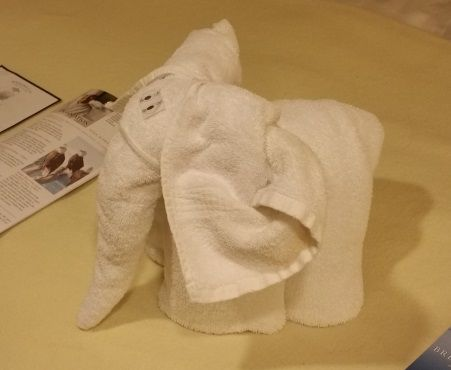
\includegraphics[width=0.5\linewidth]{./images/blog-series/xmr-crypto-luigi1111/rand-image.jpg}
\end{figure}

Until next time!

